\documentclass[twoside]{book}

% Packages required by doxygen
\usepackage{fixltx2e}
\usepackage{calc}
\usepackage{doxygen}
\usepackage[export]{adjustbox} % also loads graphicx
\usepackage{graphicx}
\usepackage[utf8]{inputenc}
\usepackage{makeidx}
\usepackage{multicol}
\usepackage{multirow}
\PassOptionsToPackage{warn}{textcomp}
\usepackage{textcomp}
\usepackage[nointegrals]{wasysym}
\usepackage[table]{xcolor}

% Font selection
\usepackage[T1]{fontenc}
\usepackage[scaled=.90]{helvet}
\usepackage{courier}
\usepackage{amssymb}
\usepackage{sectsty}
\renewcommand{\familydefault}{\sfdefault}
\allsectionsfont{%
  \fontseries{bc}\selectfont%
  \color{darkgray}%
}
\renewcommand{\DoxyLabelFont}{%
  \fontseries{bc}\selectfont%
  \color{darkgray}%
}
\newcommand{\+}{\discretionary{\mbox{\scriptsize$\hookleftarrow$}}{}{}}

% Page & text layout
\usepackage{geometry}
\geometry{%
  a4paper,%
  top=2.5cm,%
  bottom=2.5cm,%
  left=2.5cm,%
  right=2.5cm%
}
\tolerance=750
\hfuzz=15pt
\hbadness=750
\setlength{\emergencystretch}{15pt}
\setlength{\parindent}{0cm}
\setlength{\parskip}{3ex plus 2ex minus 2ex}
\makeatletter
\renewcommand{\paragraph}{%
  \@startsection{paragraph}{4}{0ex}{-1.0ex}{1.0ex}{%
    \normalfont\normalsize\bfseries\SS@parafont%
  }%
}
\renewcommand{\subparagraph}{%
  \@startsection{subparagraph}{5}{0ex}{-1.0ex}{1.0ex}{%
    \normalfont\normalsize\bfseries\SS@subparafont%
  }%
}
\makeatother

% Headers & footers
\usepackage{fancyhdr}
\pagestyle{fancyplain}
\fancyhead[LE]{\fancyplain{}{\bfseries\thepage}}
\fancyhead[CE]{\fancyplain{}{}}
\fancyhead[RE]{\fancyplain{}{\bfseries\leftmark}}
\fancyhead[LO]{\fancyplain{}{\bfseries\rightmark}}
\fancyhead[CO]{\fancyplain{}{}}
\fancyhead[RO]{\fancyplain{}{\bfseries\thepage}}
\fancyfoot[LE]{\fancyplain{}{}}
\fancyfoot[CE]{\fancyplain{}{}}
\fancyfoot[RE]{\fancyplain{}{\bfseries\scriptsize Generated by Doxygen }}
\fancyfoot[LO]{\fancyplain{}{\bfseries\scriptsize Generated by Doxygen }}
\fancyfoot[CO]{\fancyplain{}{}}
\fancyfoot[RO]{\fancyplain{}{}}
\renewcommand{\footrulewidth}{0.4pt}
\renewcommand{\chaptermark}[1]{%
  \markboth{#1}{}%
}
\renewcommand{\sectionmark}[1]{%
  \markright{\thesection\ #1}%
}

% Indices & bibliography
\usepackage{natbib}
\usepackage[titles]{tocloft}
\setcounter{tocdepth}{3}
\setcounter{secnumdepth}{5}
\makeindex

% Custom commands
\newcommand{\clearemptydoublepage}{%
  \newpage{\pagestyle{empty}\cleardoublepage}%
}

\usepackage{caption}
\captionsetup{labelsep=space,justification=centering,font={bf},singlelinecheck=off,skip=4pt,position=top}

%===== C O N T E N T S =====

\begin{document}

% Titlepage & ToC
\pagenumbering{alph}
\begin{titlepage}
\vspace*{7cm}
\begin{center}%
{\Large Calendrier \\[1ex]\large 13.\+0 }\\
\vspace*{1cm}
{\large Generated by Doxygen 1.8.13}\\
\end{center}
\end{titlepage}
\clearemptydoublepage
\pagenumbering{roman}
\tableofcontents
\clearemptydoublepage
\pagenumbering{arabic}

%--- Begin generated contents ---
\chapter{Class Index}
\section{Class List}
Here are the classes, structs, unions and interfaces with brief descriptions\+:\begin{DoxyCompactList}
\item\contentsline{section}{\textbf{ color\+\_\+writer$<$ Palette, Color $>$} }{\pageref{classcolor__writer}}{}
\end{DoxyCompactList}

\chapter{File Index}
\section{File List}
Here is a list of all files with brief descriptions\+:\begin{DoxyCompactList}
\item\contentsline{section}{\textbf{ ameltek.\+cpp} }{\pageref{ameltek_8cpp}}{}
\end{DoxyCompactList}

\chapter{Class Documentation}
\section{color\+\_\+writer$<$ Palette, Color $>$ Class Template Reference}
\label{classcolor__writer}\index{color\+\_\+writer$<$ Palette, Color $>$@{color\+\_\+writer$<$ Palette, Color $>$}}
\subsection*{Public Member Functions}
\begin{DoxyCompactItemize}
\item 
\textbf{ color\+\_\+writer} (Palette palette, Color \&color)
\item 
{\footnotesize template$<$class Vertex\+Or\+Edge $>$ }\\void \textbf{ operator()} (std\+::ostream \&out, const Vertex\+Or\+Edge \&v) const
\end{DoxyCompactItemize}


\subsection{Constructor \& Destructor Documentation}
\mbox{\label{classcolor__writer_a01986d9b2a5e01e9ab7a00a015ab143e}} 
\index{color\+\_\+writer@{color\+\_\+writer}!color\+\_\+writer@{color\+\_\+writer}}
\index{color\+\_\+writer@{color\+\_\+writer}!color\+\_\+writer@{color\+\_\+writer}}
\subsubsection{color\+\_\+writer()}
{\footnotesize\ttfamily template$<$class Palette , class Color $>$ \\
\textbf{ color\+\_\+writer}$<$ Palette, Color $>$\+::\textbf{ color\+\_\+writer} (\begin{DoxyParamCaption}\item[{Palette}]{palette,  }\item[{Color \&}]{color }\end{DoxyParamCaption})\hspace{0.3cm}{\ttfamily [inline]}}



\subsection{Member Function Documentation}
\mbox{\label{classcolor__writer_a636afacb83e8fc901d94aed9bd1c0117}} 
\index{color\+\_\+writer@{color\+\_\+writer}!operator()@{operator()}}
\index{operator()@{operator()}!color\+\_\+writer@{color\+\_\+writer}}
\subsubsection{operator()()}
{\footnotesize\ttfamily template$<$class Palette , class Color $>$ \\
template$<$class Vertex\+Or\+Edge $>$ \\
void \textbf{ color\+\_\+writer}$<$ Palette, Color $>$\+::operator() (\begin{DoxyParamCaption}\item[{std\+::ostream \&}]{out,  }\item[{const Vertex\+Or\+Edge \&}]{v }\end{DoxyParamCaption}) const\hspace{0.3cm}{\ttfamily [inline]}}



The documentation for this class was generated from the following file\+:\begin{DoxyCompactItemize}
\item 
\textbf{ ameltek.\+cpp}\end{DoxyCompactItemize}

\chapter{File Documentation}
\section{ameltek.\+cpp File Reference}
\label{ameltek_8cpp}\index{ameltek.\+cpp@{ameltek.\+cpp}}
{\ttfamily \#include $<$boost/graph/adjacency\+\_\+list.\+hpp$>$}\newline
{\ttfamily \#include $<$boost/graph/bipartite.\+hpp$>$}\newline
{\ttfamily \#include $<$boost/graph/graphviz.\+hpp$>$}\newline
{\ttfamily \#include $<$vector$>$}\newline
{\ttfamily \#include $<$random$>$}\newline
{\ttfamily \#include $<$cassert$>$}\newline
{\ttfamily \#include $<$algorithm$>$}\newline
{\ttfamily \#include $<$iostream$>$}\newline
Include dependency graph for ameltek.\+cpp\+:
\nopagebreak
\begin{figure}[H]
\begin{center}
\leavevmode
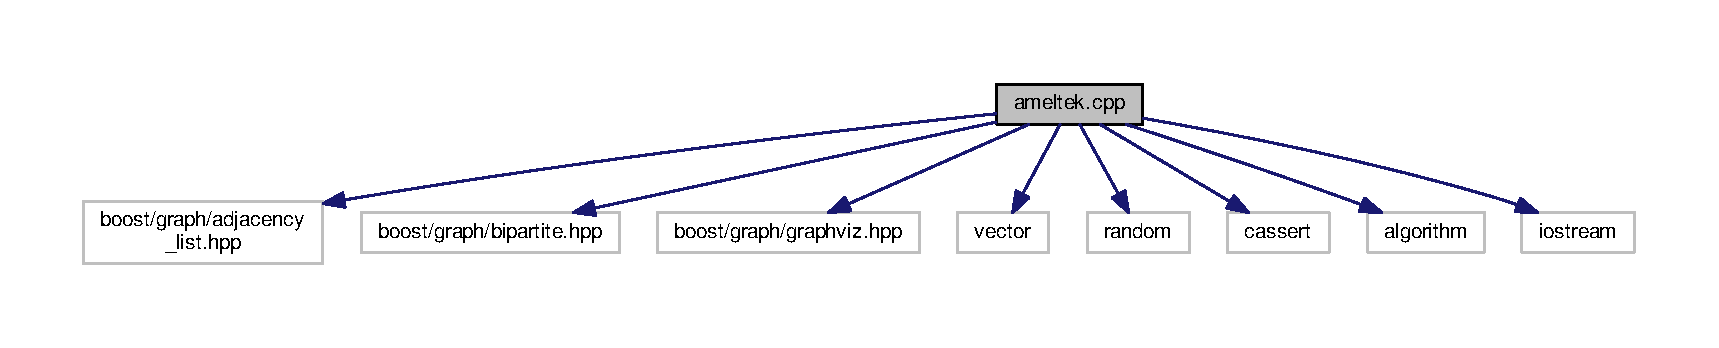
\includegraphics[width=350pt]{ameltek_8cpp__incl}
\end{center}
\end{figure}
\subsection*{Classes}
\begin{DoxyCompactItemize}
\item 
class \textbf{ color\+\_\+writer$<$ Palette, Color $>$}
\end{DoxyCompactItemize}
\subsection*{Typedefs}
\begin{DoxyCompactItemize}
\item 
typedef adjacency\+\_\+list$<$ vecS, vecS, undirectedS, no\+\_\+property $>$ \textbf{ Graph}
\end{DoxyCompactItemize}
\subsection*{Functions}
\begin{DoxyCompactItemize}
\item 
void \textbf{ random\+\_\+graph} (\textbf{ Graph} \&g, int nb\+\_\+vertex, int perc)
\item 
int \textbf{ coloration} (const \textbf{ Graph} \&g, vector$<$ int $>$ \&color)
\item 
int \textbf{ main} ()
\end{DoxyCompactItemize}


\subsection{Typedef Documentation}
\mbox{\label{ameltek_8cpp_a277ad082907fab85e9bfcfe2947dc70e}} 
\index{ameltek.\+cpp@{ameltek.\+cpp}!Graph@{Graph}}
\index{Graph@{Graph}!ameltek.\+cpp@{ameltek.\+cpp}}
\subsubsection{Graph}
{\footnotesize\ttfamily typedef adjacency\+\_\+list$<$vecS, vecS, undirectedS, no\+\_\+property$>$ \textbf{ Graph}}



\subsection{Function Documentation}
\mbox{\label{ameltek_8cpp_aabbf89358df096c183be2bdd715c3052}} 
\index{ameltek.\+cpp@{ameltek.\+cpp}!coloration@{coloration}}
\index{coloration@{coloration}!ameltek.\+cpp@{ameltek.\+cpp}}
\subsubsection{coloration()}
{\footnotesize\ttfamily int coloration (\begin{DoxyParamCaption}\item[{const \textbf{ Graph} \&}]{g,  }\item[{vector$<$ int $>$ \&}]{color }\end{DoxyParamCaption})}

\mbox{\label{ameltek_8cpp_ae66f6b31b5ad750f1fe042a706a4e3d4}} 
\index{ameltek.\+cpp@{ameltek.\+cpp}!main@{main}}
\index{main@{main}!ameltek.\+cpp@{ameltek.\+cpp}}
\subsubsection{main()}
{\footnotesize\ttfamily int main (\begin{DoxyParamCaption}{ }\end{DoxyParamCaption})}

\mbox{\label{ameltek_8cpp_ae57e42e360348ab6f9fd7018a0941cab}} 
\index{ameltek.\+cpp@{ameltek.\+cpp}!random\+\_\+graph@{random\+\_\+graph}}
\index{random\+\_\+graph@{random\+\_\+graph}!ameltek.\+cpp@{ameltek.\+cpp}}
\subsubsection{random\+\_\+graph()}
{\footnotesize\ttfamily void random\+\_\+graph (\begin{DoxyParamCaption}\item[{\textbf{ Graph} \&}]{g,  }\item[{int}]{nb\+\_\+vertex,  }\item[{int}]{perc }\end{DoxyParamCaption})}


%--- End generated contents ---

% Index
\backmatter
\newpage
\phantomsection
\clearemptydoublepage
\addcontentsline{toc}{chapter}{Index}
\printindex

\end{document}
